\section{Auswertung}
\label{sec:Auswertung}
\subsection{Vorbereitung}
Für die Vorbereitung soll das Dispersionsgebiet und das Auflösungsvermögen für die beiden 
verwendeten Wellenlängen bestimmt werden. Diese Größen können mit den Gleichungen \eqref{??}[Lena 7 und 8] berechnet werden.
Die Ergebnisse sind Tabelle \ref{tab:Vorbereitung} aufgelistet.
\FloatBarrier
\begin{table}
    \centering
    \caption{Dispersionsgebiet und Auflösungsvermögen für die beiden Wellenlängen.}
    \label{tab:Vorbereitung}
    \begin{tabular}{c c c}
        \toprule
        Wellenlänge $\lambda$ / $\SI{}{\nano\meter}$&Auflösungsvermögen $A$& Dispersionsgebiet $\Delta \lambda$ / $\SI{}{\pico\meter}$\\
        \midrule
        rot $\num{643.8}$&$\num{2.09e5}$&$\num{27.0}$\\
        blau $\num{480.0}$&$\num{2.85e5}$&$\num{48.9}$\\
        \bottomrule
    \end{tabular}
\end{table}
\FloatBarrier
Die Quantenzahlen und die mit Gleichung \eqref{??}[Lena 5] berechneten Landéfaktoren sind in Tabelle \ref{tab:Quantenzahlen} 
aufgelistet.
\FloatBarrier
\begin{table}
    \centering
    \caption{Quantenzahlen und Landéfaktoren der einzelnen Zustände.}
    \label{tab:Quantenzahlen}
    \begin{tabular}{c c c c c}
        \toprule
        Zustand&S&L&J&$g_{\text{j}}$\\
        \midrule
        $^1\text{P}_1$&0&1&1&1\\
        $^1\text{D}_1$&0&2&2&1\\
        $^3\text{S}_1$&1&0&1&2\\
        $^3\text{P}_1$&1&L&1&$\num{1.5}$\\
        \bottomrule
    \end{tabular}
\end{table}
\FloatBarrier
Die Landéfaktoren $g_{\text{ij}}$ der Übergänge werden mit der Gleichung \eqref{eq:Landeübergang} bestimmt.
\begin{equation}
    \label{eq:Landeübergang}
    g_{\text{ij}} = m_{\text{i}}g_{\text{i}} - m_{\text{j}}g_{\text{j}}
\end{equation}
Der Übergang des roten Lichtes ist $^1\text{P}_1 \rightarrow ^1\text{D}_1$ und für das 
blau Licht ist der Übergang $^3\text{S}_1 \rightarrow ^3\text{P}_1$.
Die Landéfaktoren $g_{\text{ij}}$ der Übergänge des roten Lichtes sind in Tabelle \ref{tab:rotÜber} und 
für das blaue Licht in Tabelle \ref{tab:blauÜber} aufgelistet.
\FloatBarrier
\begin{table}
    \centering
    \caption{Landéfaktoren der Zustände und Übergänge des roten Lichtes.}
    \label{tab:rotÜber}
    \begin{tabular}{c| c c| c c| c c}
        \toprule
        Übergang&\multicolumn{2}{c|}{Zustand i}&\multicolumn{2}{c|}{Zustand i}&\\
                &\multicolumn{2}{c|}{$^1\text{P}_1$}&\multicolumn{2}{c|}{$^1\text{D}_1$}&\\
        \midrule
        &$m_\text{i}$&$g_\text{i}$&$m_\text{j}$&$g_\text{j}$&$\Delta m $&$g_{\text{ij}}$\\
        \midrule
        \multirow{3}{*}{$\pi$}&1&\multirow{3}{*}{1}&1&\multirow{3}{*}{1}&\multirow{3}{*}{0}&\multirow{3}{*}{0}\\
        &0&&0&&&\\
        &-1&&-1&&&\\
        \hline
        \multirow{3}{*}{$\sigma^-$}&2&\multirow{3}{*}{1}&1&\multirow{3}{*}{1}&\multirow{3}{*}{-1}&\multirow{3}{*}{1}\\
        &1&&0&&&\\
        &0&&-1&&&\\
        \hline
        \multirow{3}{*}{$\sigma^+$}&0&\multirow{3}{*}{1}&1&\multirow{3}{*}{1}&\multirow{3}{*}{1}&\multirow{3}{*}{-1}\\
        &-1&&0&&&\\
        &-2&&-1&&&\\
        \bottomrule
    \end{tabular}
\end{table}
\begin{table}
    \centering
    \caption{Landéfaktoren der Zustände und Übergänge des blau Lichtes.}
    \label{tab:rotÜber}
    \begin{tabular}{c| c c| c c| c c}
        \toprule
        Übergang&\multicolumn{2}{c|}{Zustand i}&\multicolumn{2}{c|}{Zustand i}&\\
                &\multicolumn{2}{c|}{$^3\text{S}_1$}&\multicolumn{2}{c|}{$^3\text{P}_1$}&\\
        \midrule
        &$m_\text{i}$&$g_\text{i}$&$m_\text{j}$&$g_\text{j}$&$\Delta m $&$g_{\text{ij}}$\\
        \midrule
        \multirow{3}{*}{$\pi$}&1&\multirow{3}{*}{$\num{1.5}$}&1&\multirow{3}{*}{2}&\multirow{3}{*}{0}&$\num{-0.5}$\\
        &0&&0&&&0\\
        &-1&&-1&&&$\num{0.5}$\\
        \hline
        \multirow{2}{*}{$\sigma^-$}&1&\multirow{2}{*}{$\num{1.5}$}&0&\multirow{2}{*}{2}&\multirow{2}{*}{-1}&$\num{1.5}$\\
        &0&&-1&&&2\\
        \hline
        \multirow{2}{*}{$\sigma^+$}&0&\multirow{2}{*}{$\num{1.5}$}&1&\multirow{2}{*}{2}&\multirow{2}{*}{1}&-2\\
        &-1&&0&&&$\num{-1.5}$\\
        \bottomrule
    \end{tabular}
\end{table}
\subsection{Bestimmung des Magnetfeldes}
Um die Magnetfeldstärke bestimmen zu können, wird diese in Abhängigkeit der Stromstärke gemessen. Die Messdaten
sind in Tabelle \ref{tab:Magnetfeldstärke} aufgelistet.
\FloatBarrier
\begin{table}
    \centering
    \caption{Magnetfeldstärke und Stromstärke für die Bestimmung einer Ausgleichsgraden.}
    \label{tab:Magnetfeldstärke}
    \begin{tabular}{c c}
        \toprule
        I / $\SI{}{\ampere}$&B / $\SI{}{\milli\tesla}$\\
        \midrule
        $\num{0.45}$&$\num{39.4}$\\
        $\num{1.02}$&$\num{83.7}$\\
        $\num{1.50}$&$\num{125.7}$\\
        $\num{2.00}$&$\num{167.7}$\\
        $\num{2.50}$&$\num{209.7}$\\
        $\num{3.00}$&$\num{246.0}$\\
        $\num{3.50}$&$\num{285.4}$\\
        $\num{4.04}$&$\num{321.6}$\\
        $\num{4.49}$&$\num{352.8}$\\
        $\num{5.02}$&$\num{380.3}$\\
        \bottomrule
    \end{tabular}
\end{table}
\FloatBarrier
Durch die Daten aus Tabelle \ref{tab:Magnetfeldstärke} wird eine Ausgleichsgrade der Form
\begin{equation*}
    \text{B}(\text{I}) = m\text{I} +b
\end{equation*}
gelegt.
Die Fitparameter sind 
\begin{equation*}
    m = \SI{76(1)}{\milli\tesla\per\ampere} \quad b = \SI{12(5)}{\milli\tesla}.
\end{equation*}
Die Messdaten und die Ausgleichsgrade sind in Abbildung \ref{fig:Magnetfeldstärke} abgebildet.
\FloatBarrier
\begin{figure}
    \centering
    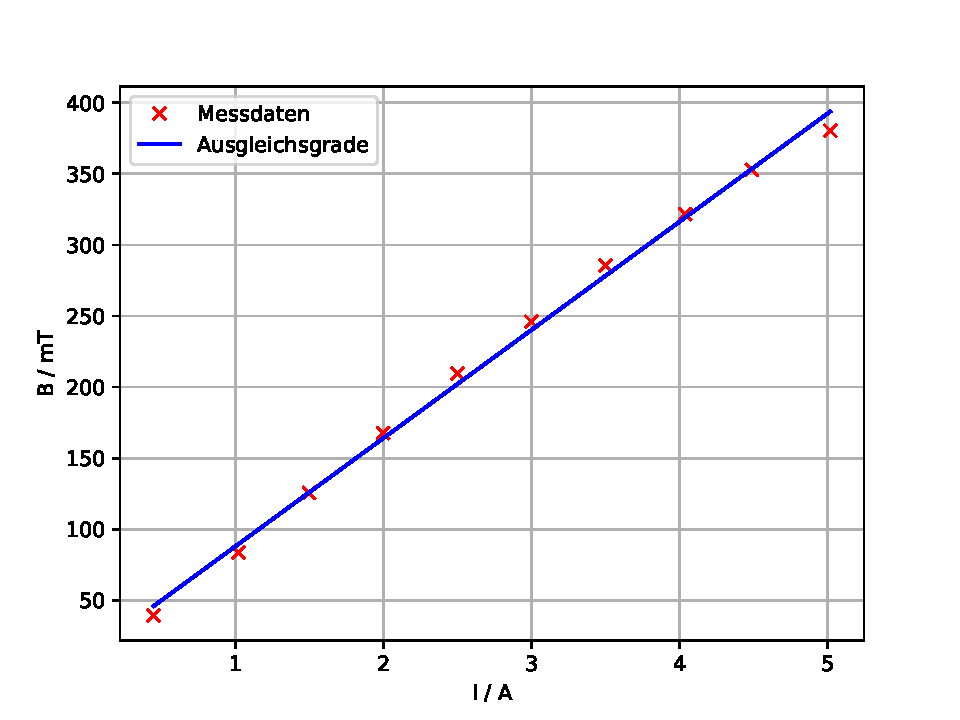
\includegraphics[width=\textwidth,keepaspectratio]{figure/B_plot.pdf}
    \caption{Messdaten und Ausgleichsgrade für die Bestimmung der Magnetfeldstärke in Abhängigkeit der Stromstärke.}
    \label{fig:Magnetfeldstärke}
\end{figure}
\FloatBarrier
